%%%%%%%%%%%%%%%%%%%%%%%%%%%%%
%   Основные пакеты
%%%%%%%%%%%%%%%%%%%%%%%%%%%%%
\documentclass[a4paper, 10pt, oneside, hidelinks]{book}
\usepackage[utf8]{inputenc}
\usepackage[T2A,OT1]{fontenc}
\usepackage{soulutf8} % дополнение к UTF8
\usepackage[russian]{babel}
% оформление полей страницы
%\usepackage{geometry}
%\geometry{verbose,a4paper,tmargin=2cm,bmargin=2cm,lmargin=2.5cm,rmargin=1.0cm}
%
\usepackage{indentfirst}
\usepackage{graphicx,lscape}
\usepackage{tabu}
%\usepackage[small,centerlast,bf]{caption2}
\usepackage[font={small}]{caption}
\DeclareCaptionLabelFormat{viadot}{\textbf{\small #1 #2.}}
\captionsetup{labelsep=space, labelformat=viadot}

\usepackage[pdftex,unicode,bookmarks=false,colorlinks=false,pdfborder={0 0 0}]{hyperref}
%\usepackage{bookmark}
\usepackage{lastpage} % для вставки количества страниц
\usepackage{needspace} % для запрета переноса страницы после слова Литература
\usepackage{enumitem} % работа со списками (интервалы и т.п.)
\usepackage{setspace} % для вертикального интервала между строк
\usepackage{makeidx} % для индекса авторов

%\usepackage{diss2018} % Стиль оформления
%\usepackage{ulem} % Способы выделения текста
%\usepackage{color} % для цветного выделения текста
%\usepackage{sectsty} % Для изменения шрифта в главах

%%%%%%%%%%%%%%%%%%%%%%%%%%%%%%%
%  Индексы GITа
%%%%%%%%%%%%%%%%%%%%%%%%%%%%%%%
% \usepackage{showidx}

%%%%%%%%%%%%%%%%%%%%%%%%%%%%%%%%
% Пакеты для таблиц и рисунков
%%%%%%%%%%%%%%%%%%%%%%%%%%%%%%%%
\usepackage{booktabs,array,tabularx}
\usepackage{longtable}
\usepackage{rotating} % поворот таблиц (и рисунков)
\usepackage{multicol} % для набора текста в несколько колонок
\usepackage{multirow} % для вертикального объединения ячеек в таблице
\usepackage{dcolumn} % для выравнивания колонок в таблицах по десятичной точке
\usepackage{float} % для удобного размещения рисунков \begin{figure}[H]
\usepackage{wrapfig} % для обтекания текстом рисунка
\usepackage{sidecap} % для side caption (размещение текста сбоку)
\usepackage{subcaption} % Для дополнительной подписи к рисунку
\sidecaptionvpos{figure}{c} % подпись сверху
%\usepackage{svg} % работа с векторной графикой
% \usepackage[off]{svg-extract} %работа с векторной графикой
%\svgsetup{clean=true}
% http://texdoc.net/texmf-dist/doc/latex/svg/svg.pdf мануал по пакету SVG
\usepackage{etoolbox} % для подсчета рисунков и таблиц
%%%%%%%%%%%%%%%%%%%%%%%%%%%%%%%%
%  Пакеты символов
%%%%%%%%%%%%%%%%%%%%%%%%%%%%%%%%
\usepackage{upgreek} % для ненаклонных греческих символов
\usepackage{amsmath} % для неразрывного дефиса  \nobreakdash
\usepackage{textcomp} % для исползьования символа градуса, лучше использовать $^\circ$
%\usepackage{latexsym}
\usepackage{wasysym} % промиле \permil0
\usepackage{amssymb} % для символа \square
\usepackage{relsize} % для увеличения размера формул в math mode

%%%%%%%%%%%%%%%%%%%%%%%%%%%%%%%%
% Рисовка графики в латехе
%%%%%%%%%%%%%%%%%%%%%%%%%%%%%%%%
\usepackage{tikz}
\usepackage{ifthen}

%%%%%%%%%%%%%%%%%%%%%%%%%%%%%%%%%
% Дополнительные команды
%%%%%%%%%%%%%%%%%%%%%%%%%%%%%%%%%
\usepackage{neisri2016}

\makeindex

\addto\captionsrussian{
	\renewcommand*{\indexname}{ad}
}



% Сжимаем в некоторых местах строки чтобы не оставалось висячих строк
\newdimen\origiwspc
\origiwspc=\fontdimen2\font% original inter word space

\newenvironment{changemargin}[2]{%
	\begin{list}{}{%
		\setlength{\topsep}{0pt}%
		\setlength{\leftmargin}{#1}%
		\setlength{\rightmargin}{#2}%
		\setlength{\listparindent}{\parindent}%
		\setlength{\itemindent}{\parindent}%
		\setlength{\parsep}{\parskip}%
		}
%
\item[]}{\end{list}}
% для списков вида 1)
\renewcommand{\labelenumi}{\theenumi)}
\DeclareUnicodeCharacter{00A0}{ }
\DeclareUnicodeCharacter{00A0}{ }
\pagestyle{headings}

%\newcommand{\dg}{\textdegree} % символ градуса
\newcommand{\dg}{$^\circ$} % круг больше чем значек градуса (использовал в сборнике молодежки 201\usepackage{neisri2016}8 года)
\newcommand{\rpm}{\raisebox{.2ex}{$\scriptstyle\pm$}} % символ плюс-минус маленький
\newcommand{\rp}{\raisebox{.2ex}{$\scriptstyle + $}} % символ плюс-минус маленький
\newcommand{\rs}[1]{\textup{\scriptsize #1}} % русские подписи в формуле
\newcommand{\Na}{\multicolumn{1}{c}{\textup{---}}} % длинное тире в таблице

%
\newenvironment{singlefigure}{\begin{figure}}{\end{figure}}


% В списке литературы номер ссылки через точку, а не в квадратных скобках
\makeatletter
\def\@biblabel#1{#1. }
\makeatother

\newcommand{\rasdel}[1]{\clearpage \hspace{1cm}\\
\begin{center}\textbf{ \LARGE #1  }\end{center} \bigskip \bigskip \bigskip \normalsize
  \addcontentsline{toc}{mmrotitle}{ \smallskip \\ \textbf{#1} \smallskip }}

\newcommand{\rasdelL}[2]{\clearpage \hspace{1cm}\\
\begin{center}\textbf{ \LARGE #1  }\end{center} \bigskip \bigskip \bigskip \normalsize
  \addcontentsline{toc}{mmrotitle}{ \smallskip \\ \textbf{#2} \smallskip }}

\newcommand{\rasdelR}[2]{\clearpage \hspace{1cm}\\
\begin{center}\textbf{ \LARGE #1  }\end{center} \bigskip \bigskip \bigskip \normalsize
  \addcontentsline{toc}{mmrotitle}{ \vspace{2cm} \bigskip \bigskip \smallskip \\ \textbf{#2} \smallskip }}



%%%%%%%%%%%%%%%%%%%%%%
%  НАЧАЛО ДОКУМЕНТА  %
%%%%%%%%%%%%%%%%%%%%%%
\begin{document}


\usefont{T2A}{cmr}{m}{n}
\captionsetup[singlefigure]{name=Fig.}

% hack for longtabu environment and odd-even page different caption
\makeatletter
\newbox\LT@oddhead
\newbox\LT@evenhead
\def\endoddhead{\LT@end@hd@ft\LT@oddhead}
\def\endevenhead{\LT@end@hd@ft\LT@evenhead}
\def\LT@head{\ifodd\c@page\LT@oddhead\else\LT@evenhead}
\makeatother


%%%%%%%%%%%%%%%%%%%%%%%%%%%%%%%%%%%%%

\maketitle
\newpage
\thispagestyle{empty}

\noindent УДК 001(571.56+571.65)(063) \\
ББК 72(2Р55)$_\rs{я}$4 \\
\indent \hspace{0.2cm} H 34

\vfill


Ответственный редактор:
чл.-корр., д.\,г.-м.\,н. \textbf{В.\,В.\,Акинин}.
\smallskip

\tolerance=500
Редакционная коллегия:
д.\,г.\,н., профессор \textbf{В.\,Н.\,Смирнов} (председатель),
к.\,б.\,н.~\textbf{О.\,П.\,Бар\-тош},
д.\,г.-м.\,н.~\textbf{А.\,С.\,Бя\-ков},
к.\,г.-м.\,н.~\textbf{И.\,С.\,Го\-лу\-бен\-ко},
к.\,г.-м.\,н.~\textbf{Е.\,Е.\,Колова},
к.\,и.\,н.~\textbf{А.\,И.\,Ле\-бе\-динцев},
д.\,б.\,н.~\textbf{В.\,П.\,Ни\-ки\-шин},
к.\,т.\,н., доцент \textbf{А.\,В.\,Сироткин},
д.\,б.\,н., доцент \textbf{А.\,А.\,Смир\-нов},
к.\,г.-м.\,н.~\textbf{И.\,М.\,Хаса\-нов},
к.\,э.\,н.~\textbf{О.\,А.\,Шарыпова}.

\bigskip
\tolerance=500
\noindent Выпуск электронной версии утвержден к печати Учёным советом СВКНИИ ДВО~РАН, протокол №~?~(???) от~??.??.2020~г.

\vfill

\begin{minipage}[t][8cm][t]{0.10\textwidth}
  \smallskip
Н 34 \hfill
\end{minipage}
\begin{minipage}[t][8cm][t]{0.85\textwidth}
  \hspace{0.6cm} \textbf{Научная молодёжь~--- Северо-Востоку России}~: Материалы
  VIII~Межрегиональной конференции молодых учёных, приуроченной к~60\nobreakdash-летнему юбилею
  Северо-Восточного комплексного научно-исследовательского института им.~Н.~А.~Шило ДВО РАН (Магадан, 26--27~ноября 2020\,г.).~---
  Магадан~: СВКНИИ ДВО РАН, 2020.~--- Вып.~8.~--- \pageref{LastPage}~с.

  \bigskip
\noindent ISBN ????-?????-????-?
  \bigskip

  \small
  \hspace{0.6cm}Представлены доклады участников VIII Межрегиональной конференции молодых учёных
  <<Научная молодёжь~--- Северо-Востоку России>>, состоявшейся 26--27~ноября
  2020\,г. в СВКНИИ~ДВО~РАН.
   Отражены фундаментальные научные исследования по следующим
   направлениям: анализ и состояние объектов окружающей среды,
   проблемы рационального природопользования,
   освоение минерально-сырьевых ресурсов,
   история освоения и развития Северо-Востока России,
   особо охраняемые природные территории и экология культуры,
   медико-экологические проблемы,
   социально-экономическое и инновационное развитие северных территорий,
   биоразнообразие и состояние экосистем,
   региональная геология и геофизические методы исследований,
   физико-математические и компьютерные методы исследований.
\end{minipage}

\vfill
\vfill
Содержат тезисы докладов молодых учёных, присланные в адрес Программного комитета конференции и прошедшие отбор на соответствие объявленной тематике. В конце сборника приведены аннотации стендовых докладов IV конкурса-выставки учащихся 2--11-х классов <<Будущие начинается сегодня>>, которые прошли проверку в системе <<Антиплагиат>> и имеют уникальность текста 70\,\% и выше.
\vfill
  \bigskip
\noindent ISBN ????-?????-????-?
\hfill \begin{minipage}[t][3cm][t]{0.38\textwidth}
\copyright СВКНИИ ДВО РАН, 2020
\end{minipage}


%\pagestyle{empty}
\pagestyle{plain}
\newpage
\tableofcontents

\clearpage
\newpage
\pagestyle{plain}


\rasdel{Геология и геофизика}
 \procTitle{Распределение скорости смещения обломочного чехла в аккумулятивных частях коллювиальных конусов в~горах Дел-Урэкчэн (Северное Приохотье), по~лихенометрическим данным}
\procAuthor{Колегов~П.\,П., Кондратьев~М.\,Н.}
\procEmail{kolegovpp@gmail.com, mkondratyev85@gmail.com}
\procOrganization{СВКНИИ ДВО РАН} \procCity{Магадан}

\makeProcTitle
\index{k@Колегов~П.\,П.}
\index{k@Кондратьев~М.\,Н.}

Рассматривая процессы склонового морфолитогенеза на территории Северного Приохотья
можно выделить следующие типы: обваливание, осыпание, десерпция, плоскостной смыв, солифлюкция.
Их изучением на Северо-Востоке Азии занимались разные исследователи с переменным успехом.
Стоит отметить работы Т.\,И.\,Каплиной посвященные криогенным образованиям
и солифлюкции в частности [4]; Э.\,Э.\,Титова описавшего типы коллювиальных образований
и их взаимосвязь с криолитозоной [9, 10]; В.\,Л.\,Суходровского разработавшего классификацию рельефообразующийх процессов криолитозоны [8].

Начиная с 2000-х гг. стали применять новые количественные и качественные методы (лихенометрия, анализ космических снимков высокого разрешения) при изучении динамики склоновых процессов,
что возобновило интерес к исследованиям в данной области. Здесь можно выделить работы В.\,Н.\,Смирнова и А.\,А.\,Галанина [1--3].

Нами проведены исследования по динамики и цикличности процессов формирующие коллювиальные конусы выноса на территории Северного Приохотья (центральная часть гор Дел-Урэкчэн), в ходе которых получены количественные данные по скорости смещения обломочного чехла (0,2--2,0\,м/год), динамического возраста (300--500\,лет) и выявлены геопространственные закономерности в размещении данных форм [5--7].

Целью данных исследований являлось выявление закономерности в распределении скорости смещения обломочного чехла в разных частях аккумулятивной зоны.

Участок исследования расположен в правом борту р.~Нельканджа (басс. р.~Армань) близ слияния с р.~Нанкалой (60°16’48”\,с.\,ш., 150°56’42”\,в.\,д.). Рельеф участка среднегорный, абсолютные отметки высот водоразделов составляют 850--900\,м, долины 530--560\,м (рис.\,1, слева). Ширина долины составляет 1500\,м, поймы до 200\,м. Форма долины U-образная. Вдоль бортов долин сохранились реликты моренные накопления последних оледенений. Склоны крутые (25--35\dg), покрытые маломощным обломочным чехлом, коренные выходы на них редки.

Для описание рельефа использовалась новая цифровая модель~--- ArcticDEM [11], которая имеет разрешение 2 м/пиксель.

Изученный нами коллювиальный конус имеет следующие морфометрические характеристики, м: длина~---  450, ширина транзитной части~---  15--25, аккумулятивной~--- 115; угол наклона транзитной части 19--26\dg, аккумулятивной~--- 12--18\dg. Превышение области питания над дистальной частью (высота морфоскульптуры)~--- 200~м. Правая часть аккумулятивной зоны (если ориентироваться вниз по склону) имеет превышение в 5~м относительно левой (анализ цифровой модели).

Обломочный чехол сложен крупнощебнистыми и мелкоглыбовым материалом в аккумулятивной зоне, и мелко-, срденещебнистые отложениями с дресвяным заполнителем в транзитной. Петрографический состав обломков представлен риолитами.

%TODO: масштабная линейка на космоснике
\begin{figure}[H]
  \centering
  \includegraphics[width=1\textwidth, page=1]{authors/Kolegov-fig.pdf}
  \caption{Цифровая модель рельефа [11] участка Нелькаджа (слева) и космоснимок фронтальной части конуса (справа). Условные обозначения: 1~--- лихеометрическая площадка и её номер, 2~--- направления транзита обломков и их скорость в м/год; на левом рисунке~--- горизонтали проведены через 50\,м, на правом~--- толстые через 10\,м, тонкие через 1\,м. На левой врезке~--- географическое положение участка исследования}
  \label{fig:kolegov-fig}
\end{figure}

В основании конуса, а также в транзитной части были заложены 4 площадки (см. рис.\,1, справа). Методика работ описана нами ранее в [5, 6], но имеются небольшие различия, а~именно были выбраны следующие параметры лихенометрической съёмки:  размер ппощадки~--- 20$\times$20\,м; лишайник индикатор~--- \textit{Rhizocarpon}~sp.; количество замеров на площадке~--- 25 случайно выбранных обломков горной породы; метод измерения~--- самый крупный таллом на обломке; точность измерения~--- 1~мм.

Данное количество замеров на одной площадке обусловлено проведёнными нами статистическими исследованиями методом Монте-Карло базы данных лихенометрической съёмки (70 площадок по 100 замеров) за 2010--2017 гг. Из генеральной совокупности измерений по каждой площадке делались 100 выборок по 25 замеров (рис. 2,\textit{а}). Средняя величина ошибки в определении возраста по сравнению с измерением 100 талломов составляет от 8 до 15\,\%, для интервала 200--500\,лет (рис. 2,\textit{б,в}).  Полученные показатели ошибки признаны допустимыми для многопрофильной съемки в аккумулятивных частях конусов выноса.



Диаметр таллома пересчитан в возраст по уравнению [6]:

$$t = 1000\cdot ln{\left(-\frac{1}{d-230}\right)}+5438,02$$

где $t$~--- возраст таллома; $d$~--- максимальный диаметр лишайника рассчитанный по убывающему логарифмическому тренду выборки из 25 измерений.

Основные показатели лихенометрического анализа приведены в таблице. Отметим, что полученные значения характерны для поверхностного слоя мощностью не~более 20~см.

\begin{figure}[H]
  \begin{center}
    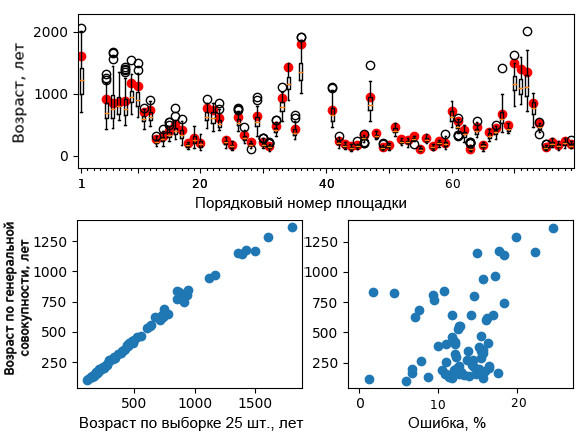
\includegraphics[width=0.8\textwidth]{authors/kolegov-fig2.jpg}
  \end{center}
  \caption{График распределения выборок (\textit{а}). Красными точками показаны истинные значения,
полученные по 100 замерам, черные боксы и кружки~--- выборки из 25 шт. Графики ошибок: \textit{б}~--- график зависимости истинных значений от выборки в 25 ед. \textit{в}~--- погрешность измерений получаемая при замере 25 шт. талломов}
  \label{fig:kolegov}
\end{figure}


\begin{changemargin}{-2cm}{-2cm}

\begin{center}
\begin{minipage}[c]{1.2\textwidth}
 \begin{table}[H]
 \begin{center}
 \caption*{\bfseries Индексы генетического разнообразия и тестов на нейтральность в исследованных популяциях}
 
 \label{tab:litvinov1}
 \medskip\small
 \begin{tabularx}{1.0\linewidth}{l c c r c r c c }
 \toprule
 %Русские юго-запад &
 \parbox[c][8em][c]{0.06\textwidth}{ \centering Про\-филь} &
 \parbox[c][8em][c]{0.10\textwidth}{ \centering Угол наклона поверхности осыпи, °} &
 \parbox[c][8em][c]{0.10\textwidth}{ \centering Длина поверхности осыпи, м} &
 \parbox[c][8em][c]{0.10\textwidth}{ \centering Площадь поверхности осыпи, м$^2$} &
 \parbox[c][8em][c]{0.08\textwidth}{ \centering Скорость транзита облом. чехла, м/год} &
 \parbox[c][8em][c]{0.12\textwidth}{ \centering Энерге\-тический потенциал, кДж} &
 \parbox[c][8em][c]{0.10\textwidth}{ \centering Удельный энергет. потенциал ($E_{\textup{уд.}}$), кДж/м$^2$} &
 \parbox[c][8em][c]{0.10\textwidth}{ \centering Удельный энергет. потенциал ($A_{\textup{уд.}}$), кДж/м$^2$}\\

 \midrule

 1 &
 30 &
 143 &
 8\,071 \hspace*{0.3cm}&
 0,67 &
 2,94$\cdot$10$^6$ &
 364,56 &
 1,70 \\
 5 &
 20 &
 194 &
 12\,620 \hspace*{0.3cm}&
 0,38 &
 4,64·10$^6$ &
 368,02 &
 0,71 \\
 8 &
 23 &
 304 &
 22\,740 \hspace*{0.3cm}&
 1,09 &
 14,62·10$^6$ &
 643,30 &
 2,30 \\
 10 &
 23 &
 108 &
 4\,014 \hspace*{0.3cm}&
 0,20 &
 0,92·10$^6$ &
 229,75 &
 0,42 \\
 11 &
 26 &
 145 &
 5\,247 \hspace*{0.3cm}&
 0,33 &
 1,77·10$^6$ &
 337,67 &
 0,76 \\
 12 &
 28 &
 118 &
 5\,000 \hspace*{0.3cm}&
 0,79 &
 1,45·10$^6$ &
 289,85 &
 1,92 \\


 \bottomrule
 \end{tabularx}
 \end{center}

 \end{table}
\end{minipage}
\end{center}
\end{changemargin}

\bigskip


\clearpage

Анализ полученных данных позволяет сделать следующие выводы:

\begin{enumerate}[noitemsep]\vspace{-8pt}
  \item Допустимо при лихенометрической съёмке производить 25 замеров талломов, при этом погрешность относительно обычной методики (100~замеров) составит 8--15\,\%;
  \item Скорость транспортировки обломков в различных частях аккумулятивной зоны варьирует от~0,17 до~0,53~м/год, при среднем значении 0,34~м/год;
  \item Динамический возраст поверхности аккумулятивной зоны варьирует от 268 до 502 лет в разных её частях;
\end{enumerate}



\begin{thebibliography}{99}
%1
\bibitem{}\BibAuthor{Галанин\,А.\,А.} Лихенометрия: современное состояние и направление развития
метода (аналитический обзор).~--- Магадан~: СВКНИИ ДВО РАН, 2002.~--- 74~с.
%2
\bibitem{}\BibAuthor{Галанин\,А.\,А.} Каменные глетчеры Северо-Востока России: строение, генезис,
возраст, географический анализ~: Дисс. $\dots$ доктора наук~: 11.00.04 / Северо-Восточный комплексный НИИ ДВО РАН.~--- Владивосток, 2009.~--- 303~с.
%3
\bibitem{}\BibAuthor{Галанин\,А.\,А., Смирнов\,В.\,Н.} Динамика гравитационных склоновых процес-
сов в горах Северного Приохотья в позднем голоцене и лихенометрическая методика их моделирования и прогноза // Геоморфология.~--- 2004.~--- №~3.~--- С.~67--75.
%4
\bibitem{}\BibAuthor{Каплина\,Т.\,И.} Криогенные склоновые процессы.~--- М.~: Наука, 1965.~--- 296~с.
%5
\bibitem{}\BibAuthor{Колегов\,П.\,П.} Динамика коллювиальных процессов в хребте Дел-Урэкчэн (Се-
верное Приохотье) на основе лихенометрических данных // Вестник СВНЦ ДВО РАН.~--- 2016.~--- №~2.~--- С.~10--18
%6
\bibitem{}\BibAuthor{Колегов\,П.\,П.} Динамика осыпей и каменных глетчеров Ольского плато (Северное Приохотье) на основании лихенометрического и фотометрического гранулометрического анализов // Вестник СВНЦ ДВО РАН.~--- 2019.~--- №~3.~--- С.~54–62.~--- DOI: 10.34078/1814-0998-2019-3-54-62.
%7
\bibitem{}\BibAuthor{Колегов\,П.\,П.} Геопространственный анализ коллювиальных конусов выноса центральной части гор Дел-Урэкчэн (Северное Приохотье) // Форум <<Наука Северо-Востока России: фундаментальные и прикладные исследования в Северной Пацифике и Арктике>>. Магадан, 5--6 марта 2020~г. / Отв. ред. Н.\,А.\,Горячев.~--- Магадан~: СВКНИИ ДВО РАН, 2020.~--- С.~41--44.
%8
\bibitem{}\BibAuthor{Суходровский\,В.\,Л.} Экзогенное рельефообразование в криолитозоне.~--- М.~:
Наука, 1979.~--- 280~с.
%9
\bibitem{}\BibAuthor{Титов\,Э.\,Э.} Скорости перемещения обломочного материала на склонах гор
Северо-Востока СССР // Вестник МГУ. География.~--- 1970.~--- №~4.~--- С.~95--98.
%10
\bibitem{}\BibAuthor{Титов\,Э.\,Э.} Строение и развитие склонов гор Северо-Востока СССР~: Автореф.
дис. $\dots$ канд. георг. наук~: 693 / Э.\,Э.\,Титов; МГУ.~--- Мoсква, 1971.~--- 35~с.

\bibitem{}ArcticDEM~--- Polar Geospatial Center.~--- 2018.~--- URL: https://www.pgc.umn.edu/data/arcticdem/ (ref. date: 20.02.2020).

\end{thebibliography}
\thispagestyle{empty}


\rasdel{Анализ и состояние объектов окружающей среды}
\procTitle{Перспективные методы биологической рекультивации на отвалах Якутии}

\procAuthor{Никифоров~А.\,А., Миронова~С.\,И., Гаврильева~Л.\,Д.}
\procEmail{aloooosha1991@mail.ru, mironova47@mail.ru, adoxa@mail.ru}
\procOrganization{НИИПЭС СВФУ} \procCity{Якутск}


\index{n@Никифоров~А.\,А.}
\index{m@Миронова~С.\,И.}
\index{g@Гаврильева~Л.\,Д.}

\makeProcTitle

Нарушение земель происходит при разработке месторождений полезных ископаемых, прокладке трубопроводов, проведении строительных, мелиоративных, лесозаготовительных, геологоразведочных, испытательных, эксплуатационных, проектно-изыскательных и иных работ, поэтому на Севере нашей страны актуальны вопросы их восстановления с применением наиболее эффективных и экономически целесообразными способами. Практическое применение на территории Республики Саха (Якутия) на нарушенных землях предприятий, занимающих алмазодобычей, угля и на россыпных месторождениях золота находятся только на опытно-экспериментальных стадиях и имеют только рекомендательный характер.  Применение старики (ветоши) для биологической рекультивации на отвалах пустых пород карьера <<Айхал>> проведена впервые на нарушенных территориях крайнего Севера. Старика (ветошь)~--- сухая прошлогодняя трава на лугах, опавшие листья. В её состав входят все не скошенные растения или отава после сенокошения, т.\,е. это луговые злаки, бобовые и разнотравье, а также реже осоковые растения.

\textbf{Целью} работы является поиск наиболее эффективных способов для восстановления нарушенных земель добывающих предприятий.

\textbf{В задачи} работы входила оценка основных факторов, воздействующих на зарастание отвалов растительностью, проведение опытно-экс\-пе\-ри\-мен\-таль\-ных работ с применением нетрадиционного материала, оценка эффективности способа, рассмотреть возможность внедрения способа в промышленных масштабах.

\textbf{Материалы и методы исследования}

Первые опытные работы по биологической рекультивации на отвалах алмазодобывающей промышленности в республике были проведены сотрудниками Института «Якутнипроалмаз» на участке площадью 2\,га, отсыпанном плодородным слоем разной мощности, испытаны 19 видов многолетних трав [1].

С развитием промышленных предприятий резко увеличилось территории нарушенных земель, который в первую очередь разрушается почвенно-растительный покров, который приводит цепочку действий, подвергающих различные изменения территории. На нарушенных территориях образуются хвостохранилища, отвалы пустых пород, карьеры и другие [2].

Начиная с 2010\,г. институтом прикладной экологии Севера СВФУ, проведены опытно-экспериментальные работы на отвалах пустых пород карьера <<Айхал>> и в 2018\,г. на отвалах угольного разреза <<Кангаласский>> с применением нетрадиционных материалов. При рекогносцировочном исследовании поверхности отвала выбрали наиболее ровную поверхность и откосы с наименьшим углом (45\dg), высота отвала 60--70 м (рис. 1).

При заложении площадки очистили от крупных валунов и глыб, размер площадки 20$\times$20\,м, на откосе 10$\times$10\,м. Вначале на опытно-экс\-пе\-ри\-мен\-таль\-ной площадке проведён посев семян из расчёта 30\,кг/га и внесение минеральных удобрений (<<Азофоска>>) из расчета 100\,кг/га действующего вещества. Сверху площадка была накрыта старикой (ветошью), закрепили тонким слоем песка и камнями (рис. 2).

Геоботаническое описание опытно-экспериментальной площадки проводилось с учетом общего проективного покрытия в процентах, средней высоты, видового состава, проективного покрытия с применением шкалы Б.\,М.\,Миркина [3].

Сбор старики (ветоши) проводился по долине р.\,Сохсолох с помощью косилок, вил и другими ручными инструментами. Для угольного разреза <<Кангаласский>> был применён прошлогодний рулон сена, который вполне подходит для проведения опытно-экспериментальных работ.

\textbf{Результаты исследований и их обсуждение}

На опытно-экспериментальной площадке в отвале пустых пород карьера <<Айхал>> среднее проективное покрытие травостоя в первый год составило 40\,\%, на второй год 50\,\%, а максимального значения достигла 80\,\%, средняя высота травостоя в первый год 3\,см, а на второй год достигла 45\,см. Видовой состав в первом году (2011\,г.) составлял в количестве от 1--2, на последующие годы увеличилось до 7\,видов (рис. 3).

\begin{figure}
  \begin{center}
    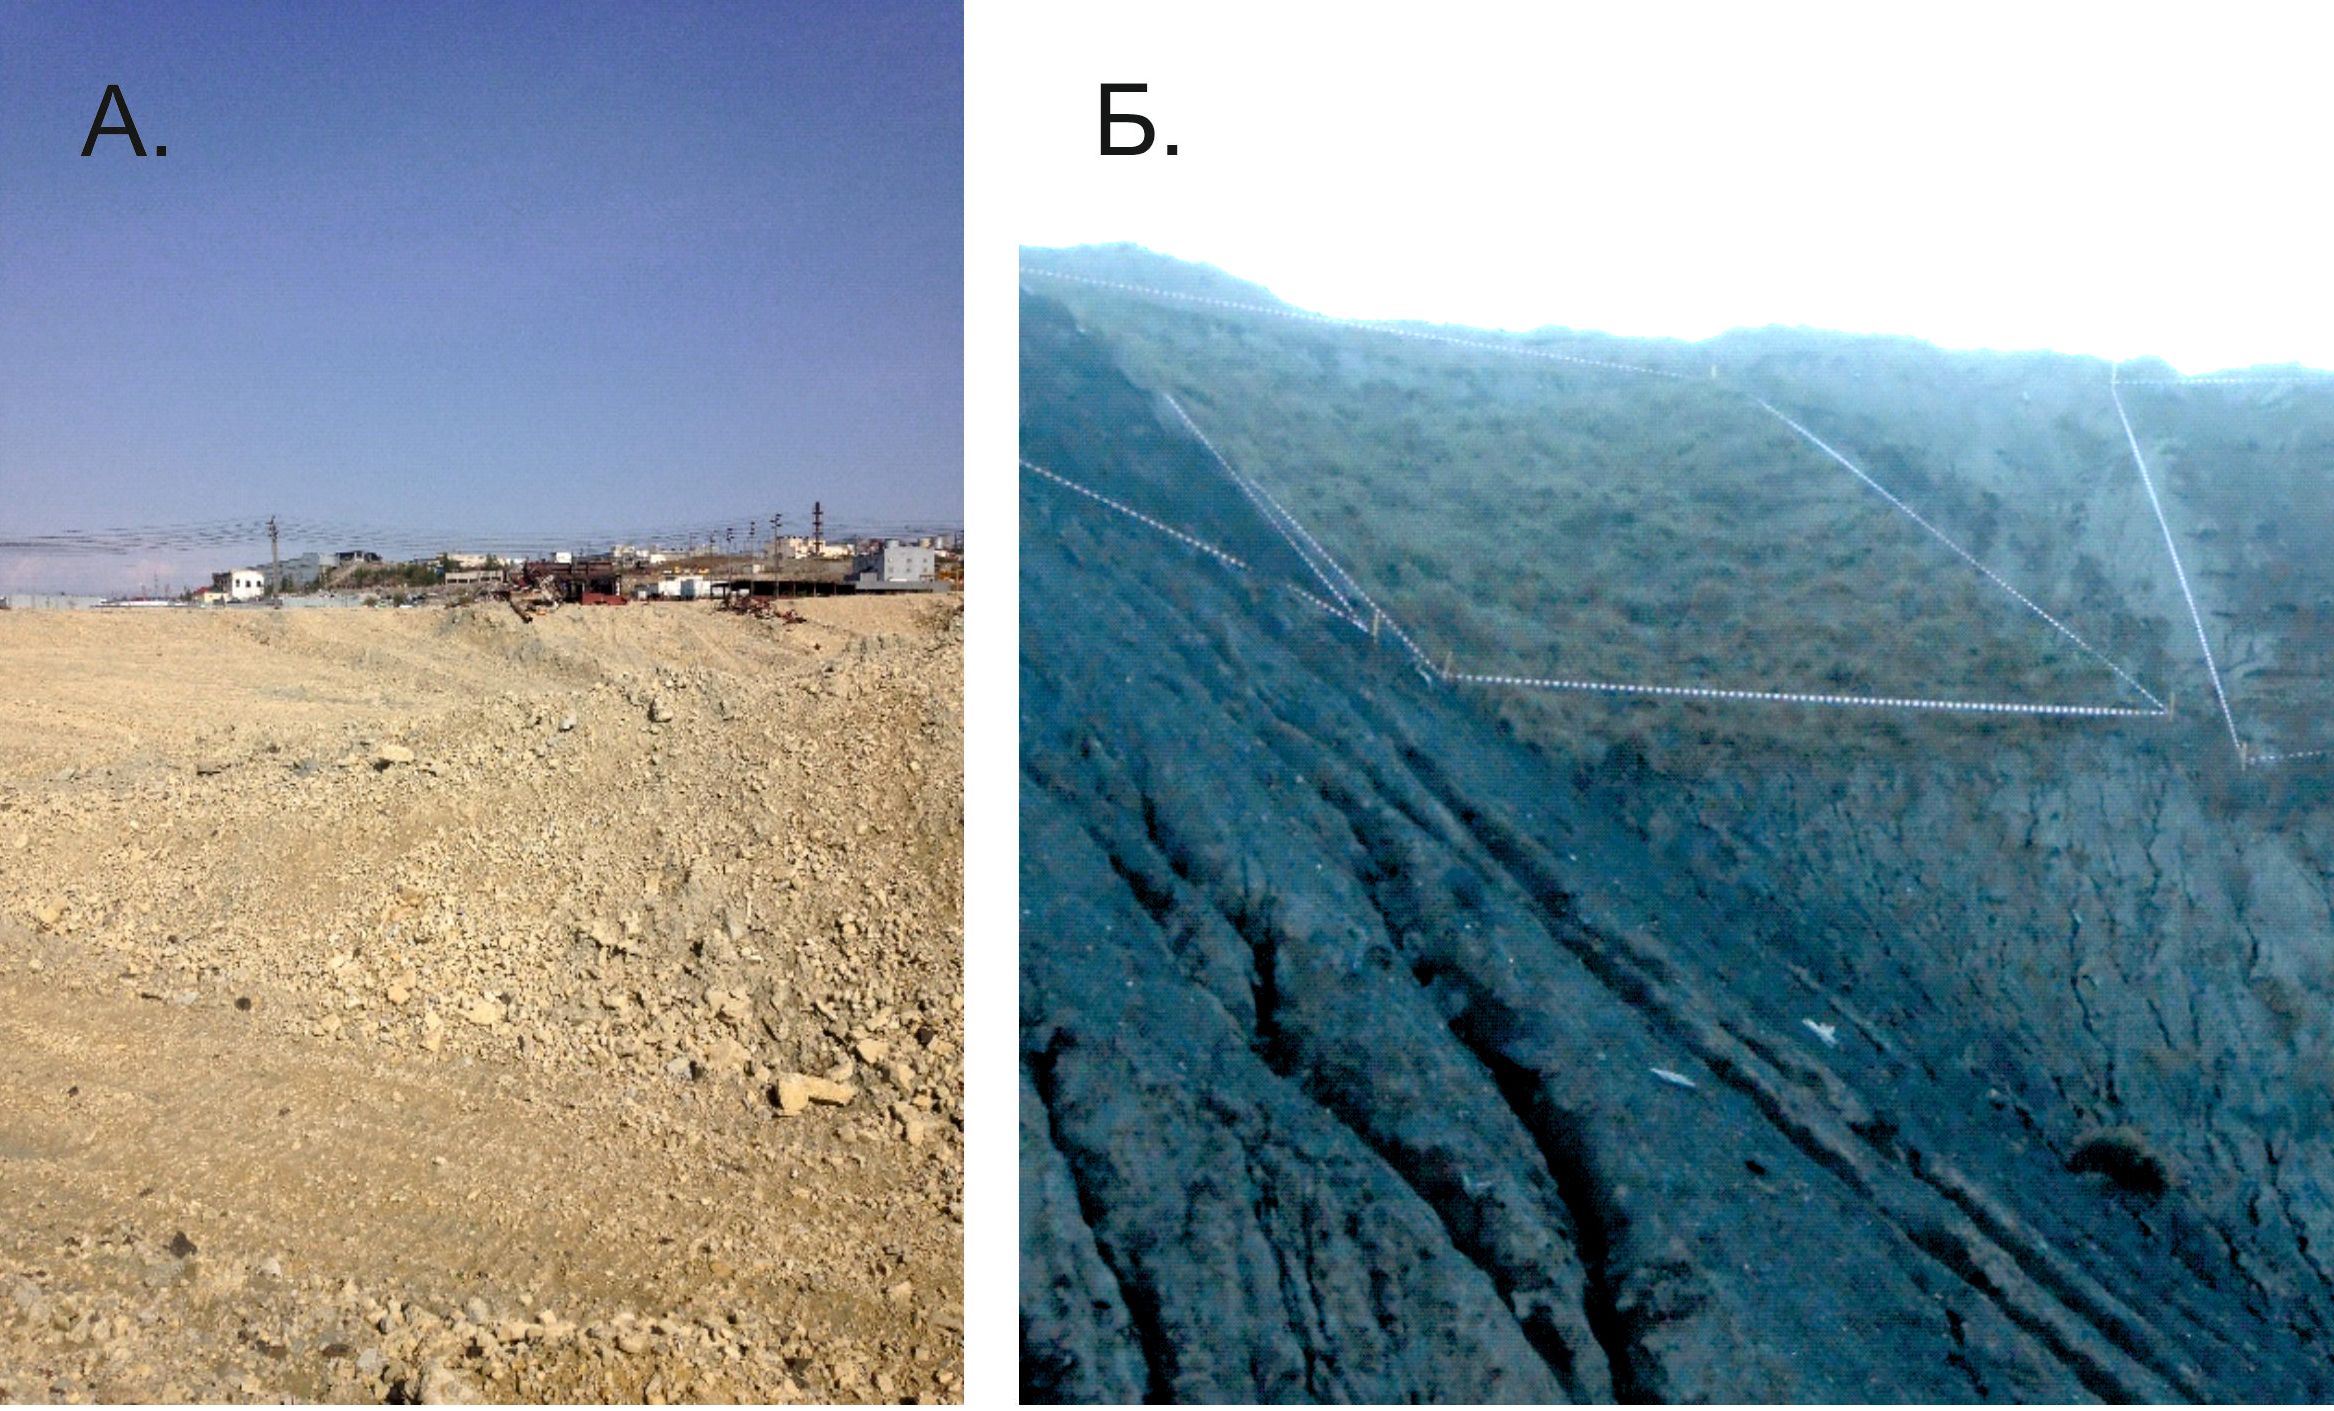
\includegraphics[width=0.9\textwidth]{authors/nekiforov-fig1.jpg}
  \end{center}
  \caption{Поверхность отвала пустых пород карьера <<Айхал>> (А) и откос отвала угольного разреза <<Кангаласский>> (Б)}
  \label{fig:nekiforov-fig1}
\end{figure}

\begin{figure}
  \begin{center}
    
\includegraphics[width=0.9\textwidth]{authors/nekiforov-fig2.jpg}
  \end{center}
  \caption{Опытно-экспериментальная площадка, накрытая старикой:
  А~--- отвал пустых пород карьера <<Айхал>>; Б~-- отвал угольного разреза <<Кангаласский>>}
  \label{fig:nekiforov-fig2}
\end{figure}

\begin{figure}
  \begin{center}
    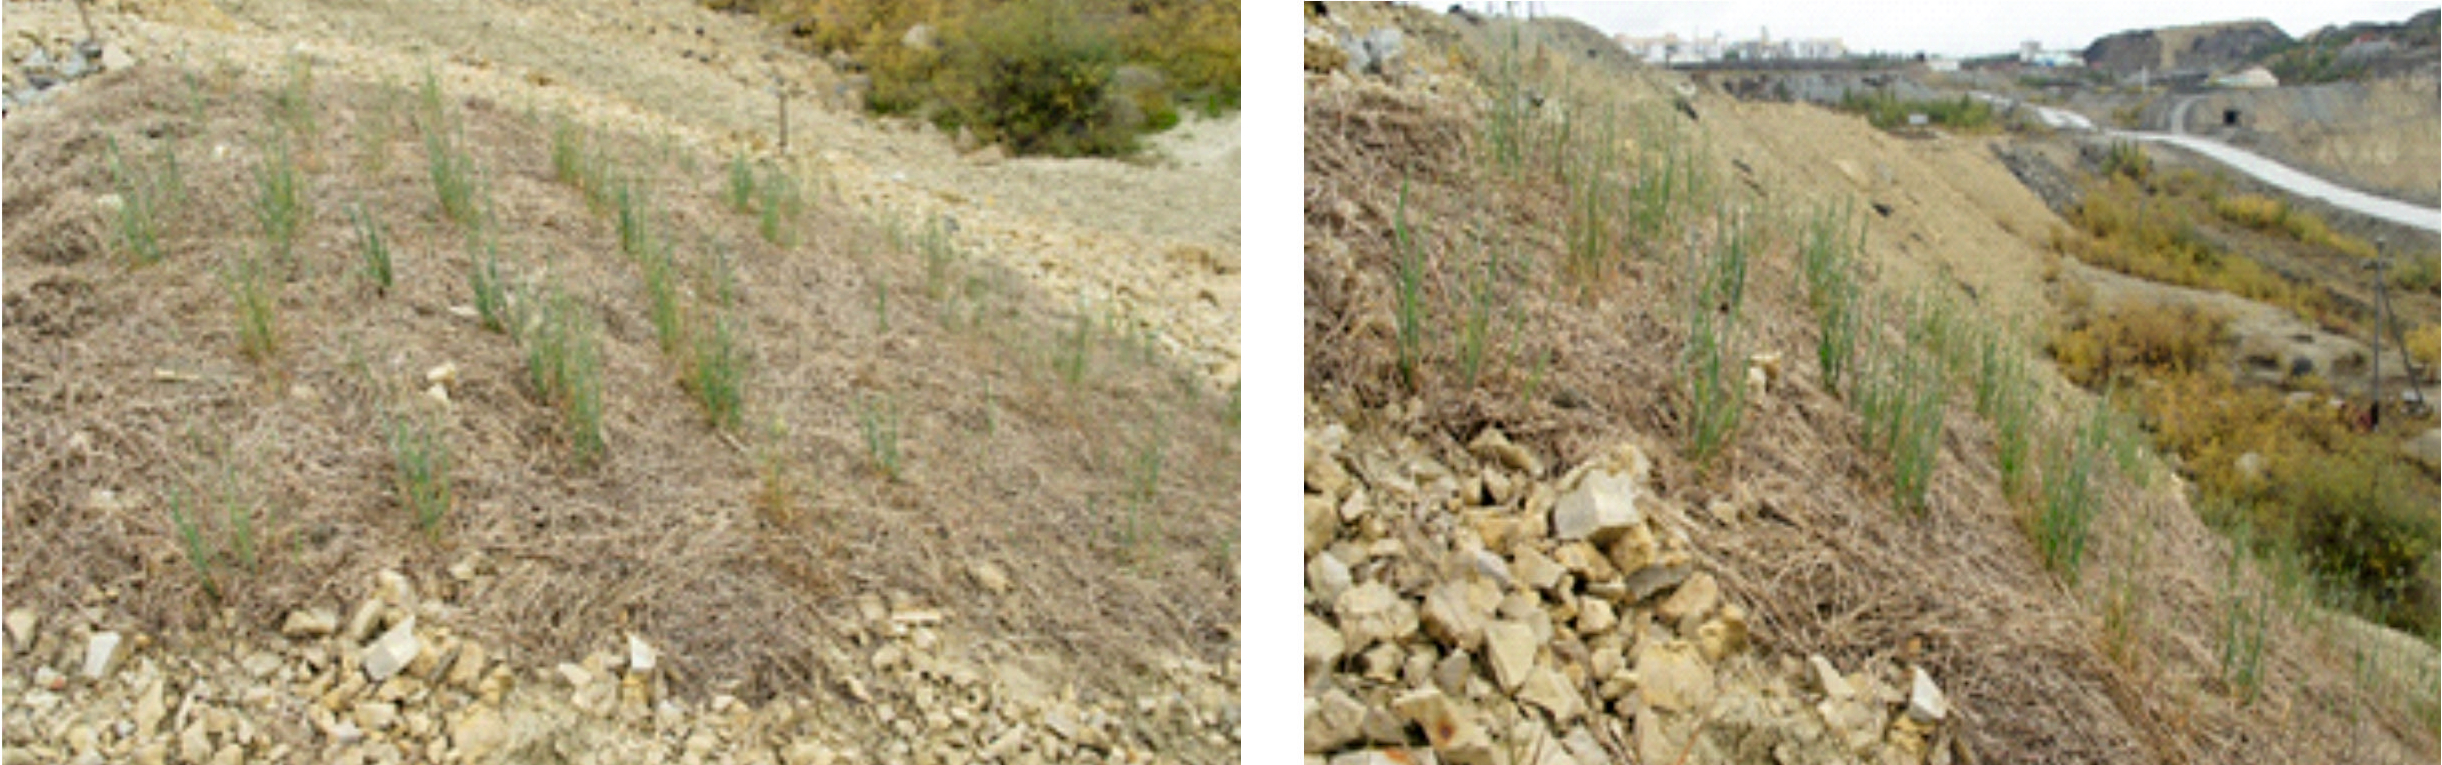
\includegraphics[width=0.9\textwidth]{authors/nekiforov-fig3.jpg}
  \end{center}
  \caption{Опытно-экспериментальная площадка с применением старики (ветоши) на отвале пустых пород карьера <<Айхал>>}
  \label{fig:nekiforov-fig3}
\end{figure}


На опытно-экспериментальной площадке в отвале угольного разреза <<Кангаласский>> среднее проективное покрытие травостоя на май месяц наблюдений составило 40--50\,\%, средняя высота 10--15\,см (май), видны всходы злаков и разнотравья. При наблюдении в июне месяце общее проективное покрытие составило 50-60\,\%, всхожесть высеянных трав составило 80\,\%, видовой состав насчитывалось до 7 видов (рис. 4).

\begin{figure}
  \begin{center}
    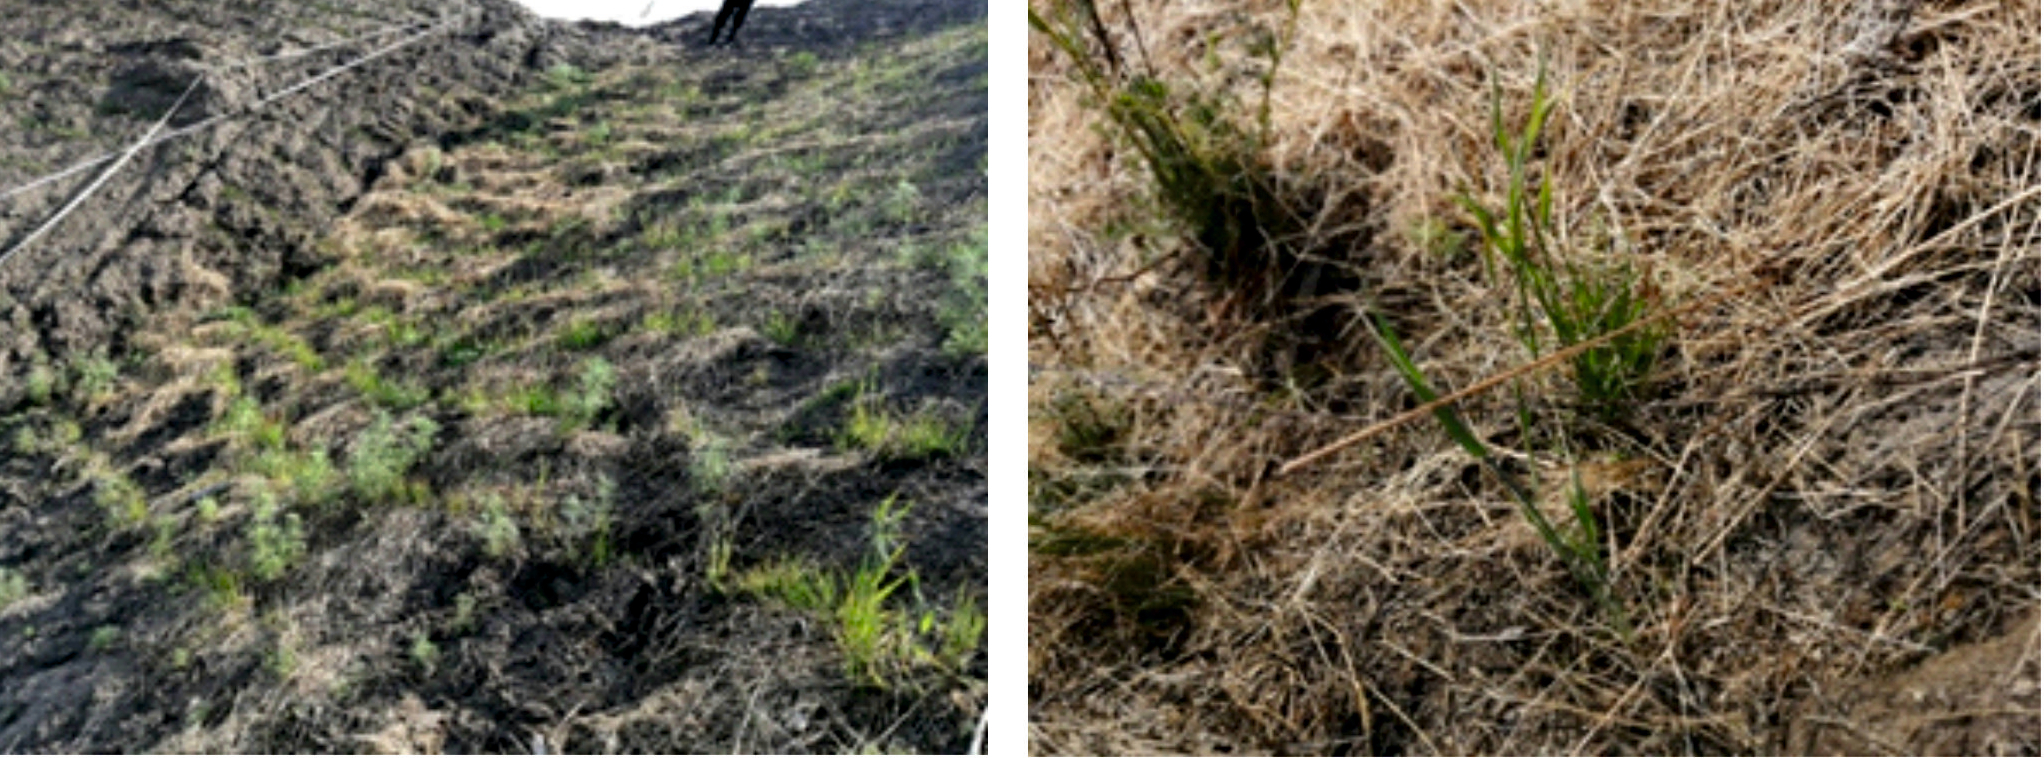
\includegraphics[width=0.9\textwidth]{authors/nekiforov-fig4.jpg}
  \end{center}
  \caption{Опытно-экспериментальная площадка с применением старики (ветоши) на отвале угольного разреза <<Кангаласский>>}
  \label{fig:nekiforov-fig4}
\end{figure}


Способ показал с перспективной стороны для внедрения в промышленных масштабах с учётом разработки технологий сбора и применения на более больших территориях. Применения старики в биологической рекультивации отвалов алмазодобычи в республике проведены впервые. В других странах этот метод применяют для других целей и в небольших объёмах только для огородов, теплицах, чаще всего в частном секторе. К применению нетрадиционного способа подтолкнуло именно условие нашего региона~--- это суровые климатические условия, экономическая целесообразность, отсутствие на данной территории потенциально плодородного слоя для отсыпки отвалов.
\clearpage
В других регионах России и мира отсыпка потенциально плодородным слоем нарушенных земель при биологической рекультивации обязательна. В нашей ситуации отсыпка плодородного слоя фактически невозможна в связи с их отсутствием, или экономической нецелесообразности их отсыпки, учитывая характер подстилающих пород траппового характера.

\textbf{Выводы}

В результате опытно-экспериментальных работ по биологической рекультивации отвалов карьера <<Айхал>> и отвалов угольного разреза <<Кангаласский>> способ применения старики (ветоши) показал наиболее эффективные результаты.

В последующем мало затратный способ можно, осуществлять повсеместно как укрывной материал без привязки к сезонным изменениям, а также в условиях отсутствия регулярного полива старика (ветошь) может, послужит задерживанием влаги и защитным слоем для всхожести семян, а при разложении питательным субстратом для роста и питания растений.

\begin{thebibliography}{99}

\bibitem{}
\BibAuthor{Лебедева\,H.\,A., Лонкунова\,А.\,Я.} Биологическая рекультивация земель, нарушенных при добыче алмазов в Якутии // Растения и промышленная среда.~--- Свердловск, 1990.~--- 71--75\,с.

\bibitem{}
ГОСТ Р 57446-2017. Наилучшие доступные технологии. Рекультивация нарушенных земель и земельных участков. Восстановление биологического разнообразия (с Поправкой).~--- Москва: Стандартинформ, 2019.~--- 47\,с.

\bibitem{}
\BibAuthor{Миркин\,Б.\,М.} Методика указания для практикума по классификации растительности методом Браун-Бланке.~--- Уфа, 1985.~--- 32\,с.
\end{thebibliography}


\rasdel{ Медицинские и экологические проблемы северных территорий}


\rasdelL{Биоразнообразие и состояние экосистем \\[04pt]
северных регионов}
{Биоразнообразие и состояние экосистем северных регионов}


\rasdelR{Вопросы истории \\[04pt]
и~социально-экономического развития северных
территорий}{Вопросы истории и~социально-экономического развития северных
территорий}



\clearpage
\phantomsection
\addcontentsline{toc}{mmrotitle}{ \smallskip \\ \textbf{Список сокращений} \smallskip }

\begin{changemargin}{-1.5cm}{-1cm}
\Large
\textbf{Список сокращений}
\vskip1.5em

\normalsize

\begin{tabular}{l c l}
  AC & --- & Арктический Совет \\
  AТР & --- & Азиатско-Тихоокеанский регион \medskip \\\medskip
  ВКП(б) & --- & Всесоюзная Коммунистическая партия (большевиков) \\
  ГАИ & --- & Группа аэронавигационной информации \\
  ГАМО & --- & Государственный архив Магаданской области \\
  ГВФ & --- & Гражданский воздушный флот\medskip \\
  ДВНЦ СО АН СССР & --- & Дальневосточный научный центр Сибирского отделения \\
  & & Академии наук СССР \\
  ДВО РАН & --- & Дальневосточное отделение Российской академии наук \medskip \\\medskip
  ИБПС ДВО РАН & --- & Институт биологических проблем Севера ДВО РАН \\
  МААН & --- & Международная ассоциация академий наук \\
  МАНК & --- & Международный акртический научный комитет \\
  МО & --- & муниципальное образование \\
  МОАГ & --- & Магаданская отдельная авиагруппа \medskip \\
  НИР & --- & научно-исследовательская работа \\
  НИЦ <<Арктика>> ДВО РАН & --- & Научно-исследовательский центр <<Арктика>> ДВО РАН\medskip\\
  ОАО & --- & объединенный авиаотряд \\
  ОЧВП & --- & Охотско-Чукотский вулканогенный пояс \medskip\\
  ПМА & --- & полевые материалы автора \medskip \\
  САФУ & --- & Северный (Арктический) федеральный университет  \\
  & & им.\,Ломоносова \\
  СВГУ & --- & Северо-Восточный государственный университет \\
  СВКНИИ ДВО РАН & --- & Северо-Восточный комплексный научно-исследовательский \\ & &
  институт ДВО РАН\\
  СВНЦ ДВО РАН & --- & Северо-Восточный научный центр ДВО РАН \\
  СО РАН & --- & Сибирское отделение Российской академии наук \medskip\\
  ткм & --- & тонно-километр \medskip \\
  УСВИТЛ & --- & Управление Северо-Восточных исправительно-трудовых\\ & & лагерей \\
  УТО & --- & учебно-тренировочный отряд \medskip \\
  ФЗ & --- & Федеральный закон \medskip \\
  ЧAО & --- & Чукотский автономный округ

\end{tabular}
\end{changemargin}
\thispagestyle{empty}

%

%  \input{sponsors}

\clearpage
\addcontentsline{toc}{mmrochapter}{ \smallskip \\ \textbf{Авторский указатель} \smallskip }
\printindex


\clearpage
\thispagestyle{empty}
\hspace{2cm}
\vfill
\begin{center}
  {Научное издание}

  \medskip
  \bigskip
  \textbf{\large Научная молодёжь~--- Северо-Востоку России}

  \medskip
  \textit{Материалы VIII Межрегиональной конференции молодых учёных, приуроченной к~60-летнему юбилею
  Северо-Восточного комплексного научно-исследовательского института им.~Н.~А.~Шило ДВО РАН\\ (Магадан,
  26--27 ноября 2020\,г.)}

  \vfill
  Выпуск 8
\end{center}
\vfill

\hspace{2cm}\\ \small
Редактор, корректор \textbf{Т.\,А.\,Фокас}\\
Компьютерная правка, верстка в \LaTeX~ \textbf{П.\,П.\,Колегова}\\
Дизайн обложки \textbf{П.\,П.\,Колегова}\\
Рисунки даны в авторском исполнении.

\vfill

\begin{center}

\includegraphics[height=30mm]{ISBN-978-5-6040134-5-8.jpg}
\end{center}


\enlargethispage{5\baselineskip}
\begin{changemargin}{-2cm}{-2cm}
\begin{center}
  \footnotesize
  Подписано в печать ??.??.2020\,г.  Формат 70$\times$108/16. Бумага
  <<Офсетная>>.\hspace*{2em}

  Гарнитура <<Таймс>>. Печать офсетная.  Усл.\,п.\,л. ??.??.
  \rule{1.1\textwidth}{.1mm}\\
  Северо-Восточный комплексный научнo-исследовательский институт им.
  Н.\,А.\,Шило ДВО РАН. \\ 685000, Магадан, ул.\,Портовая, 16.
\end{center}
\end{changemargin}


%%%%%%%%%%%%%%%%%%%%%%%%%%%%%%%%%%%%%%




\end{document}
%%%%%%%%%%%%%%%%%%%%%
%  КОНЕЦ ДОКУМЕНТА  %
%%%%%%%%%%%%%%%%%%%%%
